\chapter{Gebruik}
\chapterpreamble

\label{chap:usage}

%
%
%
\section{Plaatsen cartridges}

Vóór het opstarten van de \pkb{P2000T} dient u beide cartridges in de \pkb{P2000T} te plaatsen. De \pkb{P2000T} heeft twee sleuven, \sleuf{1} en \sleuf{2} genoemd. De zwart-oranje cartridge dient in \sleuf{1} geplaatst te worden en de zwart-wit cartridge in \sleuf{2} (zie \cref{fig:placement-cartridges}. De beide pinnetjes van de DIP schakelaar op de oranje-zwart cartridge dienen in de beneden-positie geplaatst te worden (eerste ROM, positie \pkb{00}; zie ook \cref{fig:cartridge-sleuf1} op pagina \pageref{fig:cartridge-sleuf1}). In de SD-kaart houder dient een SD-kaartje geplaatst te zijn.

\begin{figure}[h!]
    \centering
    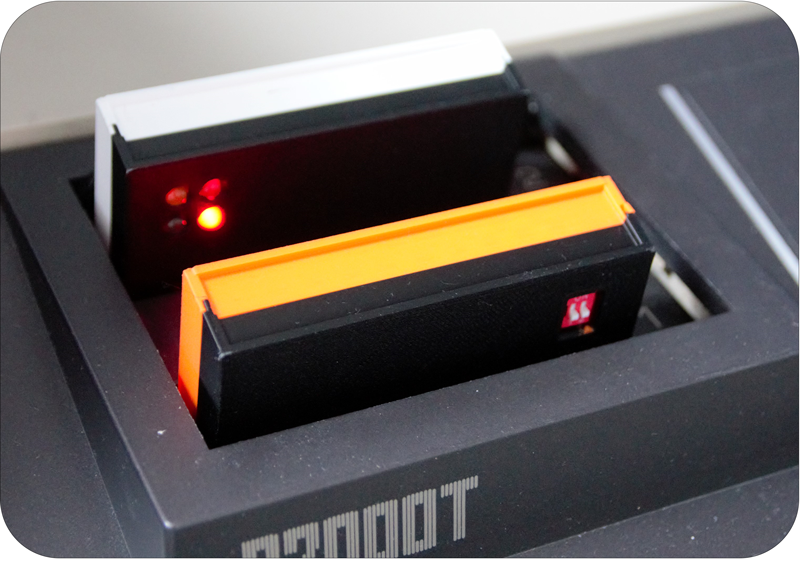
\includegraphics[width=0.50\textwidth]{img/placement-cartridges.png}
    \caption{Plaatsing van de cartridges in de P2000T.}
    \label{fig:placement-cartridges}
\end{figure}

Indien de cartridges correct geplaatst zijn, zet dan de \pkb{P2000T} aan. De \launcher zal nu opgestart worden en automatisch verbinding proberen te maken met de SD-kaart. Indien er succesvol verbinding gemaakt kan worden met de SD-kaart zal op het scherm enkele technische details over de SD-kaart getoond worden (zie \cref{fig:screenshot-boot}).

\begin{figure}[h!]
    \centering
    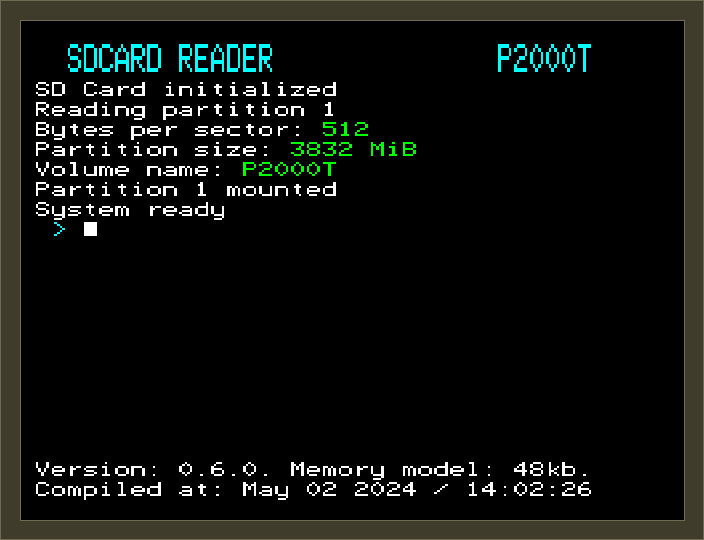
\includegraphics[width=0.99\textwidth]{img/boot.png}
    \caption{Opstartscherm van de SD-kaart lezer. De gebruiker bevindt zich nu in de \launcher omgeving.}
    \label{fig:screenshot-boot}
\end{figure}

\index{volumenaam}
\index{opstartscherm}

Het opstartscherm toont het aantal bytes per sector (\pkgr{512} bytes), de grootte van de partitie (\pkgr{3832 MiB}) en de volumenaam (\pkgr{P2000T}). De volumenaam wordt rechtsboven in het scherm nogmaals herhaald in cyaan. Dit is eventueel handig als u meerdere SD kaartjes gebruikt welke verschillende volumenamen hebben. Onderaan het scherm staat het versienummer, (\pkb{0.6.0}), het geheugenmodel\footnote{Zie ook \cref{sec:memory-model} op pagina \pageref{sec:memory-model}.} van de \pkb{P2000} en de compilatietijd. Het versienummer en de compilatietijd zijn nuttig om bugs in de software te rapporteren aan de ontwikkelaar.\footnote{Dit kan middels het aanmaken van een ``Issue'' in de Github repository: \url{https://github.com/ifilot/p2000t-sdcard}.}

Na de regel met \pkb{System ready} treft u de opdrachtregel aan. Deze regel begint met \pkc{>} gevolgd door een knipperend blokje. Middels de opdrachtregel kunt u instructies invoeren in de \pkb{P2000T} welke u afsluit door op \pkb{ENTER} te drukken. De \product zal uw instructie proberen te interpreteren en indien de instructie herkend wordt zal deze uitgevoerd worden. Bij een onbekende of ongeldige instructie zal er een foutmelding getoond worden, zoals te zien in \cref{fig:invalid-command}.

\begin{figure}[h!]
    \centering
    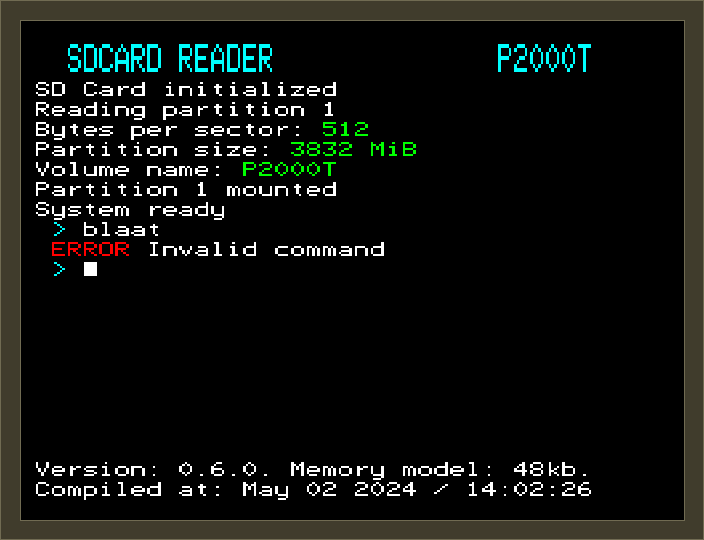
\includegraphics[width=0.99\textwidth]{img/invalid_command.png}
    \caption{Foutmelding bij het invoeren van een ongeldige instructie.}
    \label{fig:invalid-command}
\end{figure}

%
%
%
\section{Navigeren}
\label{sec:navigate}

\index{navigeren}
\index{ls}
\index{instructie!ls}

Wanneer de \pkb{P2000T} met de SD-kaart cartridge is opgestart komt u terecht in de hoofdmap (root). Vanuit hier kunt u verder navigeren naar een gewenste subfolder. Om te kijken welke bestanden en folders er zich in de hoofdmap bevinden gebruikt u de instructie \pkb{ls}. Deze instructie staat voor \textbf{list} en laat de inhoud van de huidige folder zien. Een voorbeeld hiervan wordt getoond in \cref{fig:screenshot-ls}.

\begin{figure}[h!]
    \centering
    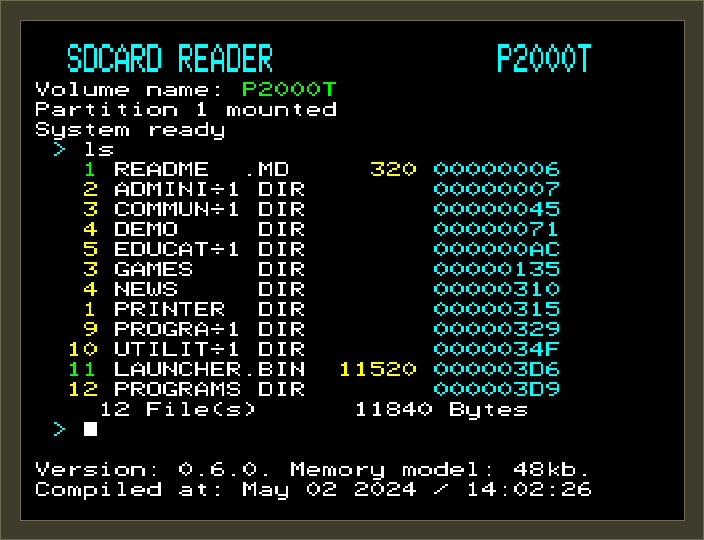
\includegraphics[width=0.99\textwidth]{img/ls.png}
    \caption{Inhoud van de hoofdmap getoond door het aanroepen van de instructie \pkb{ls}.}
    \label{fig:screenshot-ls}
\end{figure}

Het \pkb{ls} commando laat vier kolommen zien. 

\begin{enumerate}[noitemsep]
    \item De eerste kolom met oplopende getallen zijn de unieke indices die toegekend worden aan elk bestand en subfolder in de huidige folder. Indices in \pkgr{groen} zijn bestanden en indices in \pky{geel} zijn subfolders. \index{indexnummer!bestand} \index{indexnummer!folder}
    \item De tweede kolom is de naam van elk bestand of subfolder. Vanwege historische redenen zijn bestandsnamen altijd 8 + 3 karakters, dat wil zeggen, 8 karakters voor de basisnaam en 3 karakters voor de extensie. Voor het FAT32 bestandssysteem is het mogelijk om een langere naam toe te kennen, maar dan zal deze naam automatisch afgekort worden. Voor folders wordt de extensie \pkb{DIR} gebruikt en staat er ook geen punt (\pkb{.}) tussen de basisnaam en de extensie. \index{bestand!basisnaam} \index{bestand!extensie}
    \item In de derde kolom wordt de bestandsgrootte in bytes weergegeven. Dit gebeurt alleen voor bestanden. Voor subfolders staat hier niets. \index{bestand!grootte}
    \item In de vierde en laatste kolom wordt het clusternummer in \pkc{cyaan} in hexadecimale notatie\footnote{Zie \cref{sec:hexnot} op pagina \pageref{sec:hexnot}.} weergegeven. Dit is de positie op de SD-kaart waar het bestand of subfolder opgeslagen staat.
\end{enumerate}

\index{cd}
\index{instructie!cd}
\index{indexnummer}

U kunt van folder wisselen door middel van de instructie: \pkb{cd<getal>}. Deze instructie staat voor \textbf{Change Directory}. Op de plaats van \pkb{<getal>} vult u het \pkb{indexnummer} in welke u reeds eerder heeft uitgelezen met \pkb{ls}. Om bijvoorbeeld naar de folder \pkb{Games} te gaan, welke index \pky{6} heeft, typt u \pkb{cd 6} of alternatief \pkb{cd6} (zonder de spatie). Zie \cref{fig:screenshot-cd6} voor een weergave.

\begin{figure}[h!]
    \centering
    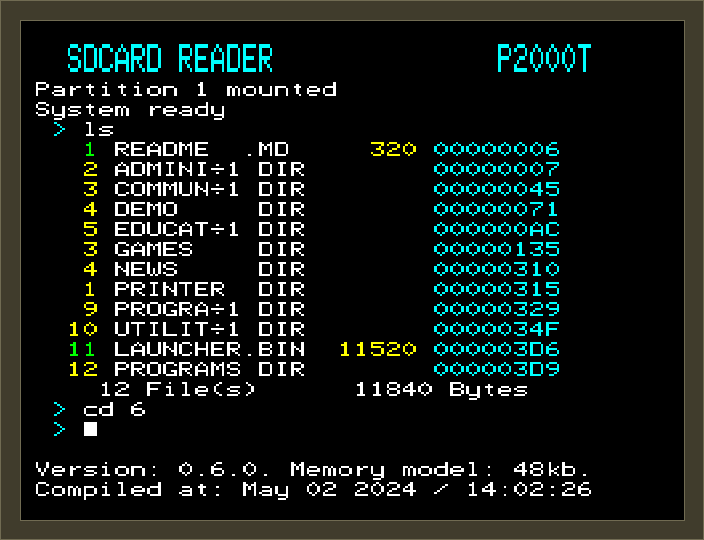
\includegraphics[width=0.99\textwidth]{img/cd6.png}
    \caption{Invoeren van de instructie \pkb{cd 6} resulteert in het navigeren naar de subfolder \pkb{Games}.}
    \label{fig:screenshot-cd6}
\end{figure}

\index{lscas}
\index{instructie!lscas}

Om de bestanden in de subfolder \pkb{Games} uit te kunnen lezen kan in principe weer de instructie \pkb{ls} gebruikt worden. Er bestaat ook een alternatief welke hier wellicht handiger is. Aangezien de subfolder \pkb{Games} voornamelijk \cas bestanden bevat die elk een header met extra informatie hebben is de instructie \pkb{lscas} wellicht nuttiger. Deze instructie zal net zoals \pkb{ls} de lijst van bestanden laten zien, maar voor \cas bestanden zal de metadata\footnote{Zie \cref{sec:cas-files} op pagina \pageref{sec:cas-files} voor meer informatie over .CAS bestanden.} uitgelezen worden en eveneens op het scherm getoond worden. Een voorbeeld van het uitvoeren van \pkb{lscas} wordt getoond in \cref{fig:screenshot-lscas}.

\begin{figure}[h!]
    \centering
    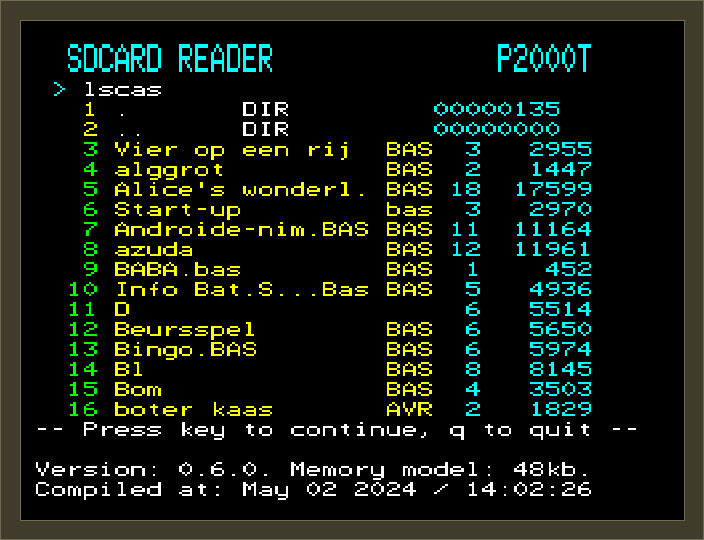
\includegraphics[width=0.99\textwidth]{img/lscas.png}
    \caption{Invoeren van de instructie \pkb{lscas} geeft een overzichtslijst van de bestanden weer waarbij voor \cas bestanden de header uitgelezen wordt.}
    \label{fig:screenshot-lscas}
\end{figure}

\begin{enumerate}[noitemsep]
    \item De eerste kolom met oplopende getallen betreffen de unieke indices die toegekend worden aan elk bestand en subfolder in de huidige folder. Indices in \pkgr{groen} zijn bestanden en indices in \pky{geel} zijn subfolders. \index{indexnummer!bestand} \index{indexnummer!folder}
    
    \item Voor \cas bestanden staat in de tweede kolom nu het label van het bestand welke bestaat uit 16 karakters. Het is belangrijk om op te merken dat dit label niet altijd overeenkomt met de originele bestandsnaam en soms is het nuttig om \pkb{ls} met \pkb{lscas} te combineren.\footnote{In plaats van \pkb{lscas} kan men ook \pkb{hexdump} gebruiken om de header van een enkel bestand uit te lezen. Voor meer informatie, zie \cref{sec:hexdump} op pagina \pageref{sec:hexdump}.}\index{bestandsnaam}
    
    \item De derde kolom bevat het bestandstype. Meestal staat hier \pky{BAS} voor BASIC bestanden, maar uiteindelijk kan de auteur van het \cas bestand hier iets anders neergezet hebben.\footnote{De \pkb{P2000T} handleiding benoemt slechts 5 soorten bestanden, zijnde \pkb{BAS}, \pkb{INT}, \pkb{SNG}, \pkb{DBL} en \pkb{FAM}. Door de jaren heen hebben verschillende auteurs hier hun eigen typen aan toegevoegd en bestaat er geen ook standaard.} \index{bestandstype}
    
    \item De vierde kolom omvat het aantal blokken in \pkc{cyaan}.\footnote{Zie \cref{sec:cas-files} op pagina \pageref{sec:cas-files} voor meer informatie over blokken in .CAS bestanden.} Elk blok correspondeert met \pkb{0x500} bytes aan data.
    
    \item In de vijfde en laatste kolom wordt de programmagrootte in \pkc{cyaan} weergegeven. Let op dat de programmagrootte verschilt van de bestandsgrootte. Dit heeft ermee te maken dat de \cas bestanden acteren als een datadrager voor de programma's.\footnote{Meer informatie over \cas bestanden is te vinden in \cref{sec:cas-files} op pagina \pageref{sec:cas-files}.}\index{programmagrootte}
\end{enumerate}

Omdat de subfolder \pkb{Games} meer dan 16 bestanden en folders bevat wordt het tonen van de lijst gepauzeerd na 16 items. Dit is zodat de gebruiker de tijd krijgt om de lijst te kunnen doorlezen. Men kan kiezen om het commando te termineren door op \pkb{q} te drukken of te continueren door op elke andere toets te drukken.

%
%
%
\section{Inladen van bestanden}
\label{sec:loading}
\index{inladen!cas}
\index{inladen!prg}
\index{cas!inladen}
\index{prg!inladen}

\index{CAS|see{cas}}
\index{PRG|see{prg}}

Er zijn twee type bestanden die opgestart kunnen worden met de \product. Het eerste type zijn \cas bestanden, welke cassetteband programma's bevatten. Het andere type is een nieuw type speciaal geintroduceerd voor de \product welke \prg bestanden zijn.\footnote{Voor meer informatie over \prg bestanden, zie \cref{sec:prg-files} op pagina \pageref{sec:prg-files}. Voor het draaien van \prg bestanden dient de \pkb{P2000T} tenminste een 16 KiB geheugenuitbreiding te hebben.} Beide bestanden kunnen opgestart worden middels het \pkb{run<nummer>} commando waarbij \pkb{nummer} refereert naar het bestandsindex.

Ter illustratie geven we hier een demonstratie voor het opstarten van het programma \pko{Fraxxon} vanaf een koude boot.\footnote{Een koude boot is wanneer de P2000T opnieuw aangezet wordt of wanneer de RESET toets is ingedrukt.} Na het opstarten gaan we eerst naar de subfolder \pkb{Games} waarna we \pko{Fraxxon} opstarten met \pkb{run 45}.\footnote{Voor het opvragen van de indices kan men de instructies \pkb{ls} of \pkb{lscas} gebruiken. Let erop dat enkel in dit voorbeeld Fraxxon op positie \pkb{45} staat. Voer dus altijd eerst \pkb{ls} of \pkb{lscas} uit voordat men \pkb{run} gebruikt.} In \cref{fig:screenshot-run-fraxon} staat het proces afgebeeld.

\begin{figure}[h!]
    \centering
    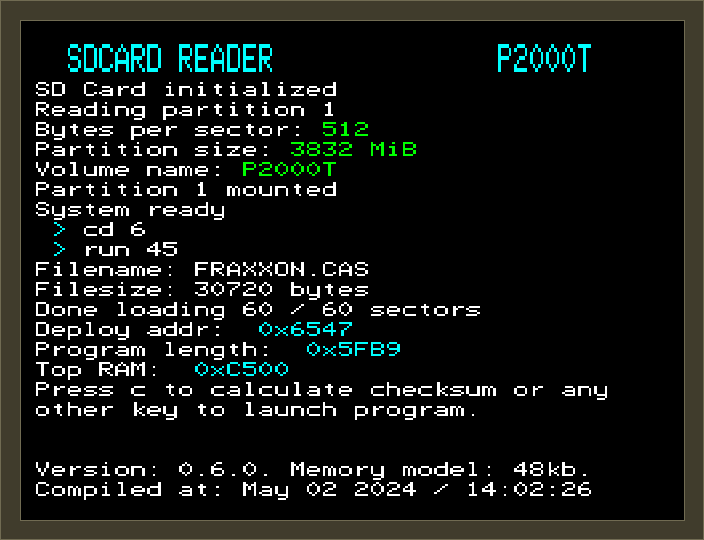
\includegraphics[width=0.99\textwidth]{img/run-fraxxon.png}
    \caption{Opstarten van het programma \pko{Fraxxon}.}
    \label{fig:screenshot-run-fraxon}
\end{figure}

\index{run}
\index{instructie!run}

Wanneer \pkb{run} wordt uitgevoerd op een \cas bestand, dan wordt op het scherm de bestandsnaam en -grootte\footnote{Dit betreft de grootte van het \cas bestand, \textbf{niet} de grootte van het daadwerkelijk programma dat \textbf{in} het \cas bestand staat.} getoond. Ook zal een tellertje gaan lopen waarin het aantal ingeladen sectoren en het totaal aantal sectoren te zien is. Zodra het programma ingeladen is wordt ook de locatie, de programmalengte en de bovenste positie in het RAM geheugen getoond. In het geval van \pko{Fraxxon} wordt het programma geplaatst op positie \pkc{0x6547}, is het programma in totaal \pkc{0x5FB9} bytes\footnote{\pkb{0x5FB9} is $24505$ in decimale notatie.} groot en is de bovenste positie in het RAM geheugen \pkc{0xC500}. Dit voorbeeld laat meteen zien dat voor dit programma een geheugenuitbreiding nodig is. Zonder geheugenuitbreiding is het hoogst alloceerbare RAM adres \pkb{0x9FFF}. Om \pko{Fraxxon} te draaien is dus tenminste een 16 KiB geheugenuitbreiding nodig.

Bij het uitvoeren van \pkb{run} op een \cas bestand wordt het programma eerst naar het RAM geheugen \textbf{van de cartridge} gekopieerd. Nadat het programma in het RAM geheugen van de cartridge is geladen kan de gebruiker kiezen om een CRC-16 checksum uit te rekenen door op de \pkb{c} toets te drukken of om het programma op te starten door op elke willekeurig andere toets te drukken. Wanneer de gebruiker een \pkb{P2000T} bezit met onvoldoende geheugen kan men ervoor kiezen om het proces af te breken door op de \pkb{RESET} toetst te drukken. Voor het uitrekenen van de CRC-16 checksum hoeft men geen geheugenuitbreiding te hebben en kan men dit altijd doen.

Als men op een willekeurig andere toets dan \pkb{c} drukt, zal het interne RAM geheugen opgeruimd worden om plaats te maken voor het programma dat op de RAM chip van de cartridge is geplaatst. Het programma wordt vervolgens automatisch opgestart. Men keert hierna niet meer terug naar het menu en dient op \pkb{RESET} te drukken wanneer men een ander programma wilt spelen. Indien het \pkb{BASIC} programma het ondersteunt kan men ook op de \pkb{SHIFT + STOP} drukken om terug te keren naar de BASIC prompt. Men zal wederom niet naar het menu terugkeren, maar het ingeladen programma staat wel nog steeds in het geheugen. Men kan dan met reguliere \pkb{BASIC} instructies\footnote{Zie ook de \pkb{P2000T} handleiding voor meer informatie} het ingeladen programma bewerken of bijvoorbeeld opslaan op een cassettebandje (met \pkb{CSAVE}).

\index{cassettebandje}
\index{tape|see{cassettebandje}}

Wanneer men op de \pkb{c} toets heeft gedrukt, dan wordt de CRC-16 checksum uitgerekend. Een voorbeeld hiervan is getoond in \cref{fig:screenshot-run-fraxon-checksum}. Deze CRC-16 checksum kan men gebruiken om bijvoorbeeld te controleren of het programma goed is ingeladen, maar ook of de \product en diens RAM geheugen goed functioneren. In het geval van \pko{Fraxxon} blijkt de CRC-16 checksum gelijk te staan aan \pkc{0x0C3F}. Meer informatie over CRC-16 checksums en waarom dat deze gebruikt worden treft men aan in \cref{sec:crc16-checksum} op pagina \pageref{sec:crc16-checksum}.

\begin{figure}[h!]
    \centering
    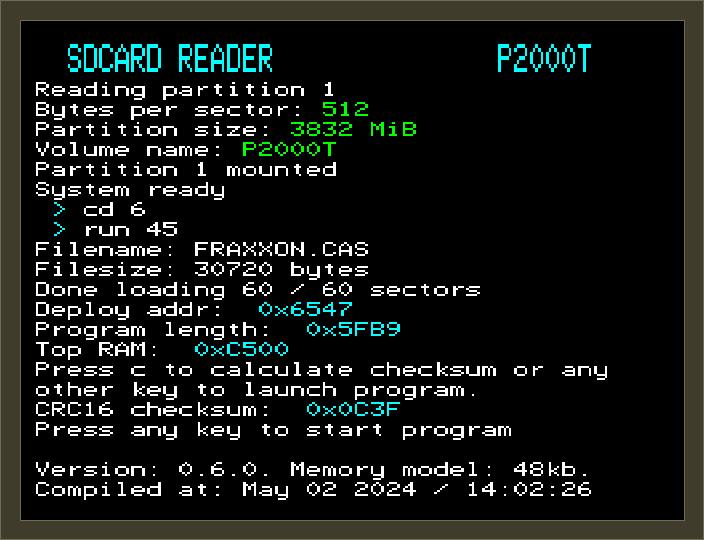
\includegraphics[width=0.99\textwidth]{img/run-fraxxon-checksum.png}
    \caption{Uitrekenen van de CRC-16 checksum van het programma \pko{Fraxxon}.}
    \label{fig:screenshot-run-fraxon-checksum}
\end{figure}

%
%
%
\section{Uitlezen van bestanden}
\label{sec:hexdump}
\index{hexdump}
\index{instructie!hexdump}

De bestanden die ingeladen en opgestart kunnen worden met de \product zijn voorzien van een header, een stukje metadata dat de inhoud van het bestand beschrijft. Om deze metadata op het scherm te tonen bestaat er de instructie \pkb{hexdump}. Deze instructie toont de eerste 120 bytes van een bestand op het scherm. Deze bytes worden getoond als een ``hexdump''. In een hexdump wordt de waarde van elke byte weergegeven in hexadecimale notatie.\footnote{Zie \cref{sec:hexnot} op pagina \pageref{sec:hexnot} voor meer informatie over hexadecimale notatie.} Wanneer de waarde van een byte $c$ zich binnen het bereik $27 \leq c \leq 127$ bevindt, dan wordt tevens aan de rechterzijde het corresponderende ASCII karakter getoond. Voor waarden buiten dit bereik wordt een \pkb{.} geprint.

\begin{figure}[h!]
    \centering
    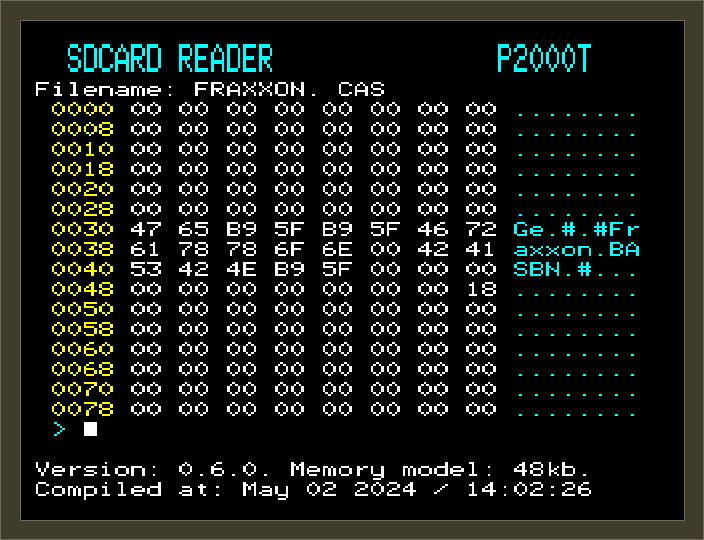
\includegraphics[width=0.99\textwidth]{img/hexdump-fraxxon.png}
    \caption{Hexdump van de eerste 120 karakters van \pkb{FRAXXON.CAS}.}
    \label{fig:screenshot-hexdump-fraxxon}
\end{figure}

In \cref{fig:screenshot-hexdump-fraxxon} is een voorbeeld van een hexdump van het bestand \pkb{FRAXXON.CAS} weergegeven. In de eerste kolom in \pky{gele} letters staat de adrespositie van de eerste karakter van elke regel in hexadecimale notatie. De adrespositie van het eerste karakter is \pkb{0x0000}. De adrespositie van het eerste karakter op de tweede regel is \pkb{0x0008} en op de derde regel \pkb{0x0010}.

In de tweede tot en met negende kolom staan de waarden van de bytes weergegeven in hexadecimale notatie. Zo kan men zien dat de byte op adrespositie \pkb{0x0030} de waarde \pkb{0x47} heeft. In de laatste kolom worden de corresponderende ASCII tekens in \pkc{cyaan} getoond. Omdat de waarde \pkb{0x47} zich in het bereik $27 \leq c \leq 127$ bevindt wordt het corresponderende ASCII teken aan de rechterzijde afgebeeld, welke de letter \pkb{G} is.

Op basis van deze hexdump kunnen we zien dat in de header de naam \pkb{Fraxxon} staat, om precies te zijn vanaf positie \pkb{0x36}. Ook kunnen we zien dat dit programma ingeladen dient te worden op adres \pkb{0x6547}, wat te lezen valt vanaf adrespositie \pkb{0x0030}.\footnote{Hierbij dient opgemerkt te worden dat bestanden groter dan 8 bits weggeschreven worden in ``little endian`` notatie. Dit staat in meer detail uitgelegd in \cref{sec:endianness} op pagina \pageref{sec:endianness}.} Op adrespositie \pkb{0x0032} treffen we de grootte van het programma aan, hetgeen \pkb{0x5FB9} bytes betreft. Tenslotte zien we op adrespositie \pkb{0x004F} dat het programma in totaal \pkb{0x18} blokken aan data bevat.\footnote{Meer informatie over de header van een \cas programma valt te lezen in \cref{sec:cas-files} op pagina \pageref{sec:cas-files}.}

%
%
%
\section{Geheugendumps}
\label{sec:memdumps}
\index{geheugendumps}

Naast het uitlezen van bestanden zoals gedemonstreerd in de vorige paragraaf is het ook mogelijk om het geheugen van de \pkb{P2000T} uit te lezen. Hierin maken we onderscheid tussen het interne RAM geheugen en het externe ROM en RAM geheugen op de cartridge. De drie instructies die we gebruiken voor het in- en uitlezen van het geheugen staan hieronder

\begin{itemize}[noitemsep]
    \item \pkb{dump<XXXX>}: Leest het interne RAM geheugen van de P2000T uit. \index{dump} \index{instructie!dump}
    \item \pkb{romdump<bXXXX>}: Leest het externe ROM geheugen op de cartridge uit. \index{romdump} \index{instructie!romdump}
    \item \pkb{ramdump<bXXXX>}: Leest het externe RAM geheugen op de cartridge uit. \index{ramdump} \index{instructie!ramdump}
\end{itemize}

Bij \pkb{dump<XXXX>} dient \pkb{<XXXX>} vervangen te worden voor het geheugenadres in hexadecimale notatie (\textbf{altijd} 4 karakters). Bij \pkb{romdump<bXXXX>} en \pkb{ramdump<bXXXX>} dient \pkb{b} vervangen te worden voor een \pkb{0} of een \pkb{1} voor de eerste of tweede bank van het externe ROM of RAM geheugen en \pkb{<XXXX>} voor het geheugenadres in hexadecimale notatie.\footnote{Zie \cref{sec:hexnot} op pagina \pageref{sec:hexnot}} De uitvoer van deze instructies is zeer vergelijkbaar met hetgeen getoond in \cref{fig:screenshot-hexdump-fraxxon}, echter zal de eerste kolom met de addressen in \pky{geel} oplopen vanaf het adres dat gebruikt is voor de instructie.

Wanneer voor \pkb{b} een andere waarde dan \pkb{1} wordt gebruikt, wordt automatisch bank \pkb{0} gekozen. Dit houdt dus ook in dat wanneer men \pkb{romdump\;0000} invoert met een spatie op de positie van \pkb{b}, er een 120-byte hexdump wordt gemaakt van bank \pkb{0} vanaf adrespositie \pkb{0x0000}.

%
%
%
\section{Overzicht instructies}

In \cref{tab:commands} wordt een overzicht getoond van alle instructies voor de \product. Let bij het invoeren van deze instructies erop dat het stukje tekst in haakblokes (\pkb{<...>}) acteert als een variabele en vervangen dient te worden voor een waarde. Voor de instructies \pkb{ls}, \pkb{lscas} en \pkb{run} is de spatie tussen de instructie en de waarde optioneel en mag deze weggelaten worden. Voor de instructies \pkb{dump}, \pkb{romdump} en \pkb{ramdump} staat er \pkr{geen} spatie tussen de instructie en het geheugenadres. Het geheugenadres \pkb{XXXX} dient ingevoerd te worden in hexadecimale notatie.\footnote{Zie \cref{sec:hexnot} op pagina \pageref{sec:hexnot}}.

\begin{table}[h!]
    \caption{Lijst van instructies. Let erop dat de haakblokjes (\pkb{<...>}) acteren als een variabele en deze vervangen dienen te worden voor een waarde.}
    \label{tab:commands}
    \centering
    \begin{tabular}{|l|p{6cm}|}
    \hline
    \textbf{Instructie}  & \textbf{Omschrijving}                                           \\ \hline\hline
    
    \texttt{ls}        & Geeft de inhoud van de huidige folder weer. \smaller (\cref{sec:navigate}) \index{instructie!ls} \index{ls}                               \\ \hline
    
    \texttt{lscas}     & Geeft de inhoud van de huidige folder weer, lees hierbij \cas bestanden in en toon de headerinformatie van deze bestanden. \smaller (\cref{sec:navigate}) \index{instructie!lscas} \index{lscas} \\ \hline
    
    \texttt{cd <getal>}       & Verander huidige folder. \smaller (\cref{sec:navigate})                         \index{instructie!cd} \index{cd} \\ \hline
    
    \texttt{run <getal>}      & Start \cas of \prg bestand op. \smaller (\cref{sec:loading})                                                  \index{instructie!run} \index{run} \\ \hline
    
    \texttt{hexdump <getal>}  & Voer een 120-byte hexdump van een bestand uit. \smaller (\cref{sec:hexdump})                          \index{instructie!hexdump} \index{hexdump} \\ \hline
    
    \texttt{fileinfo <getal>} & Print informatie zoals bestandspositie en grootte van een bestand.                           \index{instructie!fileinfo} \index{fileinfo}  \\ \hline
    
    \texttt{ledtest}           & Laat de lees en schrijf LED lampjes knipperen voor elk een halve seconde.                   \index{instructie!ledtest} \index{ledtest} \\ \hline
    
    \texttt{stack}             & Laat de positie van de stack pointer zien in hexadecimale notatie.                   \index{instructie!stack} \index{stack} \\ \hline
    
    \texttt{dump<XXXX>}             & Voer een 120-byte hexdump uit van het \pkr{interne} RAM geheugen startend vanaf positie \pkb{0xXXXX}. \smaller (\cref{sec:memdumps})                   \index{instructie!dump} \index{dump} \\ \hline
    
    \texttt{romdump<bXXXX>}             & Voer een 120-byte hexdump uit van het \pkr{cartridge} ROM geheugen voor bank \pkb{b} vanaf positie \pkb{0xXXXX}. \smaller (\cref{sec:memdumps})                 \index{instructie!romdump} \index{romdump}  \\ \hline
    
    \texttt{ramdump<bXXXX>}             & Voer een 120-byte hexdump uit van het \pkr{cartridge} RAM geheugen voor bank \pkb{b} vanaf positie \pkb{0xXXXX}. \smaller (\cref{sec:memdumps})                   \index{instructie!ramdump} \index{ramdump} \\ \hline
    \end{tabular}
\end{table}